\documentclass[../main.tex]{subfiles}
\graphicspath{
    {"../img/"}
    {"img/"}
}

\begin{document}
Ostatnio zastanawialiśmy się nad taką sytuacją, że mieliśmy operator $P_a(x)$ i on miał być zwężający. \[
    P_a(x): X\to X \text{ - zwężający }
.\]
\[
    c\in X: \left\{ c,P_a(c),P_a(P_a(c)) \to \tilde x(a) \right\}\text{, gdzie }P(\tilde x(a)) = \tilde x(a)
.\]
\begin{proof}
    Chcemy pokazać, że \[
        \underset{\varepsilon >0}{\forall} . \underset{\delta > 0}{\exists}. \underset{a'}{\forall}  d(a,a') < \delta \implies d(\tilde x(a),\tilde x(a')) < \varepsilon
    .\]
    Wiemy, że $P_a$ - ciągła ze względu na $a$:
    \begin{equation}\label{eq:del}
        \underset{\varepsilon_1>0}{\forall}. \underset{\delta_1>0}{\exists} .\underset{a'}{\forall} d(a,a') < \delta_1 \implies d(P_a, P_{a'}) < \varepsilon
    \end{equation}
    Wiemy, że $\underset{c'\in X}{\forall}$ ciąg $\left\{ c',P_{a'}(c'), P_{a'}(P_{a'}(c'))\ldots \right\} \to \tilde x(a')$
    Ale, jeżeli przyjmiemy za $c = \tilde x(a')$, to ciąg:
    \[
        \left\{ \tilde x(a'),P_{a}(\tilde x(a')), P_{a}(P_{a}(\tilde x(a'))) \right\} \to \tilde x(a)
    .\]
    Ale z zasady banacha wiemy, że jeżeli $P_{a}$ - zwężający, to
    \[
        d(\tilde x(a),x_0) \le \frac{1}{1-q} d(x_1,x_0)
    .\]
    Wybierzmy $x_0 = \tilde x(a')$. Wówczas
    \begin{align*}
        d(\tilde x(a),\tilde x(a')) &\le \frac{1}{1-q}d(P_a(\tilde x(a')) ,\tilde x(a')) =\\
        &= \frac{1}{1-q} d(P_a(\tilde x(a')), P_{a'}(\tilde x(a')))
    .\end{align*}
    \begin{pytanie}
        Jak ten obiekt ma się do $d(P_{a},P_{a'})$?\\
        \[
            d(P_a,P_{a'}) = \underset{x\in X}{\sup} \quad d(P_a(x), P_{a'}(x))
        .\]
    \end{pytanie}
        Więc, jeżeli $d(P_{a'},P_a)<\varepsilon_1$, to znaczy, że $d(P_a(\tilde x(a')),P_{a'}(\tilde x(a'))) < \varepsilon_1$\\
        \[
            \text{Czyli } d(\tilde x(a),\tilde x(a')) \le \frac{1}{1-q} \varepsilon_1
        .\]
        Czyli jeżeli otrzymamy $\varepsilon_1$, to biorąc $\varepsilon_1$ taki, że $\varepsilon_1 \frac{1}{1-q}<\varepsilon$ i znajdujemy $\delta_1$ z zależności \ref{eq:del} i wiemy, że jeżeli
       \[
           d(a',a) < \delta_1 \implies d(\tilde x(a'),\tilde x(a))<\varepsilon \quad\Box
       .\]
\end{proof}
\begin{przyklad}
    (odwzorowanie zwężające)\\
    \[
        \int \frac{dx(t)}{dt} = f(t,x), x(t_0) = x_0
    .\]
    Wiemy, że $x(t)$ jest punktem stałym odwzorowania
    \[
        P(g) = x_0 + \int_{t_0}^{t} f(s,g(s)) ds \implies g_0,P(g_0),P(P(g_0))\ldots\to x(t)
    .\]
    \[
        \frac{dx}{dt} = t+x, x(0) = 0
    .\]
    \[
        f(t,x) = t+x. t_0 = 0, x_0 = 0
    .\]
    Czy $f$ jest lipszycowalna?
    \[
        \underset{t\in [a,b]}{\forall} \Vert t+x - (t+x') \Vert = \Vert x-x' \Vert = 1 \Vert x-x' \Vert \implies L = 1
    .\]
    Czyli jest. Policzymy kilka wyrazów ciągu
    \[
        \underset{x^0(t)}{g_0},\underset{x^1(t)}{P(g_0)}, \underset{x^2(t)}{P(P(g_0))},\ldots
    .\]
    \begin{align*}
        &x^0(t) = x_0(t) = 0\\
        &x^1(t) = P(x^0(t)) = P(0) = 0 + \int_0^t f(s,x^0(s))ds = \int_0^t s ds = \frac{t^2}{2}\\
        &x^2(t) = P(x^1(t)) = P(\frac{t^2}{2}) = 0 + \int_0^t f(s,x^1(s)) ds = \int_0^t (s+\frac{s^2}{2})ds = \frac{t^2}{2} + \frac{t^3}{2 \times 3}\\
        &x^3(t) = P(x^2(t)) = 0 + \int_0^t \left(s+\frac{s^2}{2}+\frac{s^3}{2\times 3} \right)ds  = \frac{t^2}{2}+\frac{t^3}{2\times 3}+\frac{t^4}{2\times 3\times 4}\\
        &\vdots\\
        &\vdots \to \infty\\
        &e^t - t - 1
    .\end{align*}
\end{przyklad}
\begin{przyklad}

    $\frac{dx}{dt} = 2tx,\quad x(0) = 1$, czyli $f(t,x) = 2tx,\quad t_0 = 0$

    dla $\underset{t\in[a,b]}{\forall} $
    \[
        \Vert 2tx - 2tx' \Vert \le \underset{t\in[a,b]}{\sup} |t| 2 \Vert x-x' \Vert
    .\] Czyli $f$ - lipszycowalna z $L = \underset{t\in[a,b]}{\sup} |t| \times 2$
    \begin{align*}
        &x^0(t) = 1\\
        &x^1(t) = P(x^0(t)) = 1 + \int_0^t f(s,1)ds = 1 + \int_0^t 2sds = 1+t^2\\
        &x^2(t) = P(x^1(t)) = 1 + \int_0^t 2s(1+s^2)ds = 1 + t^2 + \frac{t^4}{2}\\
        &x^3(t) = P(x^2(t)) = 1 + \int_0^t 2s(1+s^2 + \frac{t^4}{2}) =  1 + t^2 + \frac{t^4}{2} + \frac{t^6}{3}\\
        &\vdots \to \infty\\
        &e^{t^2}
    .\end{align*}
\end{przyklad}
\begin{przyklad}
    \[
        \frac{d}{dt} \begin{bmatrix} x_1(t)\\x_2(t) \end{bmatrix} = \begin{bmatrix} x_2(t)\\-x_1(t) \end{bmatrix} ,
        x_1(0) = 0, x_2(0) =  1
    .\]
    \[
        f(t,x) = f(t,\begin{bmatrix} x_1\\x_2 \end{bmatrix} = \begin{bmatrix} 0&1\\-1&0 \end{bmatrix} \begin{bmatrix} x_1\\x_2 \end{bmatrix}
    .\]
    \begin{align*}
        &x^0(t) = \begin{bmatrix} x_1^0(t)\\x_2^0(t) \end{bmatrix} = \begin{bmatrix} 0\\1 \end{bmatrix}\\
        &x^1(t) = P(x^0(t)) = \begin{bmatrix} 0\\1 \end{bmatrix} + \int_0^t \begin{bmatrix} 1\\-0 \end{bmatrix} ds = \begin{bmatrix} 0\\1 \end{bmatrix} + \begin{bmatrix} t\\0 \end{bmatrix} = \begin{bmatrix} t\\1 \end{bmatrix}\\
        &x^2(t) = P\left(\begin{bmatrix} x_1^1\\x_1^2 \end{bmatrix} \right) = P\left( \begin{bmatrix} t\\1 \end{bmatrix}  \right)  = \begin{bmatrix} 0\\1 \end{bmatrix} + \int_0^1 \begin{bmatrix} 1\\-s \end{bmatrix} ds = \begin{bmatrix} 0\\1 \end{bmatrix} +\begin{bmatrix} t\\-\frac{t^2}{2} \end{bmatrix} = \begin{bmatrix} t\\1-\frac{t^2}{2} \end{bmatrix}\\
        &x^3 = P\left( \begin{bmatrix} x_1^2\\x_2^2 \end{bmatrix}  \right) = P\left( \begin{bmatrix} t\\1-\frac{t^2}{2} \end{bmatrix}  \right) = \begin{bmatrix} 0\\1 \end{bmatrix} + \int_0^t \begin{bmatrix} 1-\frac{s^2}{2}\\-s \end{bmatrix} ds = \begin{bmatrix} t-\frac{t^3}{2\times 3}\\1-\frac{t^2}{2} \end{bmatrix}\\
        &\vdots \to \infty\\
        &\begin{bmatrix} \sin{t}\\ \cos{t} \end{bmatrix}
    .\end{align*}
    \begin{figure}[h]
        \centering
        \includegraphics[width=0.8\textwidth]{fig_29}
        \caption{}
        \label{fig:fig_29}
    \end{figure}
\end{przyklad}

\pagebreak
\begin{tw}
    Jeżeli odwzorowania
        \begin{align*}
            &t\in [a,b]\to A(t)\\
            &t\in [a,b]\to b(t)
        .\end{align*}
        Gdzie $A(t)\in L(x,x), b(t) : \mathbb{R}^1\to X$ są ciągłe, to równanie
        \[
            \frac{d}{dt}x(t) = A(t)x(t) + b(t),\quad x(t_0) = x_0
        .\]
        Ma dla dowolnych $t_0\in[a,b], x_0\in X$ jednoznacznie określone rozwiązanie na $t\in]a,b[$\\
        Czym to się różni od twierdzenia o jednoznaczności warunku Cauchy? Nie ma tutaj mowy o żadnej lipszycowalności. Zawężono za to klasę funkcji występującej w równaniu.\\
        Zamiast $]t_0-\varepsilon,t_0+\varepsilon[\times \mathcal{O}$, mamy $]a,b[ \times X$
\end{tw}
\begin{proof}
    Chcemy sprawdzić, czy $f(t,x) = A(t) x(t)+b(t)$ spełnia warunek Lipschitza. Wiemy, że  $A(t)$ i $b(t)$ są ciągłe na przedziale domkniętym $[a,b]$.
    Zatem, istnieje $\underset{t\in[a,b]}{\sup} \Vert b(t) \Vert = C$, a $A: X\to X$ i $A$ jest liniowe zatem istnieje norma tego odwzorowania
    \[
        \underset{t\in[a,b]}{\sup} \Vert A(t) \Vert = L
    .\]
    Zatem
    \[
        \underset{t\in[a,b]}{\forall} \Vert A(t)x + b(t) - (A(t) x' + b(t) \Vert = \Vert A(t)(x-x') \Vert \le \underset{t\in[a,b]}{\sup} \Vert A(t) \Vert \Vert x-x' \Vert = L \Vert x-x' \Vert
    .\]
    Z twierdzenia o jednoznaczności wiemy, że istnieją przedziały
    $]t_0-\varepsilon,t_0+\varepsilon[$ oraz $\mathcal{O} = K(x_0,r_2)$ takie, że dla
    \begin{equation}\label{eq:esion}
        \varepsilon = min\left\{|a-t_0|,r_1,\frac{r_2}{M},|b-t_0|,\frac{1}{L} \right\}
    \end{equation}
    Gdzie $r_1,r_2$ były takie, że na zbiorze $K(t_0,r_1)\times K(x_0,r_2)$ funkcja $f(t,x)$ była ograniczona.
    Zależy nam na tym, aby w warunku \ref{eq:esion} wyeliminować $r_2$\\
    Ale $\Vert A(t)x + b(t) \Vert \le \Vert A(t)x\Vert + \Vert b(t) \Vert$ dla $x\in K(x_0,r_2)$
    \begin{align*}
        &= \Vert A(t)x \Vert + C \le L\Vert x \Vert + C = \\
        &= L\Vert x-x_0+x_0 \Vert +C \le\\
        &\le L \Vert x-x_0 \Vert + L \Vert x_0 \Vert  + C\le\\
        &\le L r_2 + L \Vert x_0 \Vert +C
    .\end{align*}




\end{proof}
\end{document}
